\section{Topology Generator for Federated IT Networks\label{sec:topologies.approach}}

To solve the limitations of existing datasets in the literature, we introduce \thecontrib, a topology generator for federated IT networks.
In this section, we present the design and architecture of \thecontrib, before detailing its implementation using Airbus' CyberRange platform\footnote{\url{https://www.cyber.airbus.com/products/cyberrange/}}.


\subsection{Approach Overview\label{sec:topologies.approach.overview}}

The core idea behind \thecontrib is to compose network topologies by selecting and connecting a set of building blocks that satisfy user-supplied constraints from a library of predefined sub-topologies.
While creating this library remains human operated, the composition of the topologies is fully automated, allowing the generation of different topologies with common characteristics.
\thecontrib is a two-step algorithm:
\begin{enumerate}
  \item \emph{Topology selection:} Use constraint programming to find all sets of sub-topologies that satisfy the user-defined constraints, based on a library of predefined sub-topologies.
  \item \emph{Topology composition:} For each set, connect the sub-topologies in a tree-like structure starting from the \emph{Master} sub-topology.
\end{enumerate}

\begin{figure}
  \centering
  \begin{subfigure}[b]{0.49\linewidth}
    \centering
    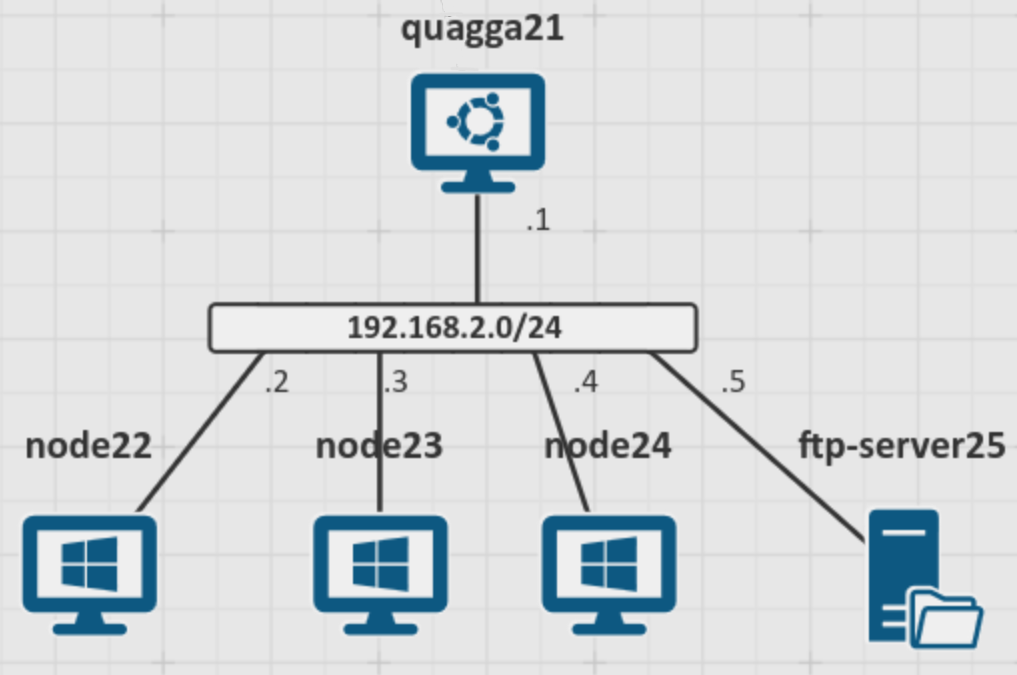
\includegraphics[width=\linewidth]{figures/sub_topology.png}
    \caption{
      Example of a sub-topology instantiated on Airbus' CyberRange, containing 3 Windows clients and 1 FTP server.
      The node labeled \texttt{quagga21} is the gateway connecting the sub-topology to the rest of the network.
      \label{fig:topologies.example}
    }
  \end{subfigure}
  \hfill
  \begin{subfigure}[b]{0.49\linewidth}
    \centering
    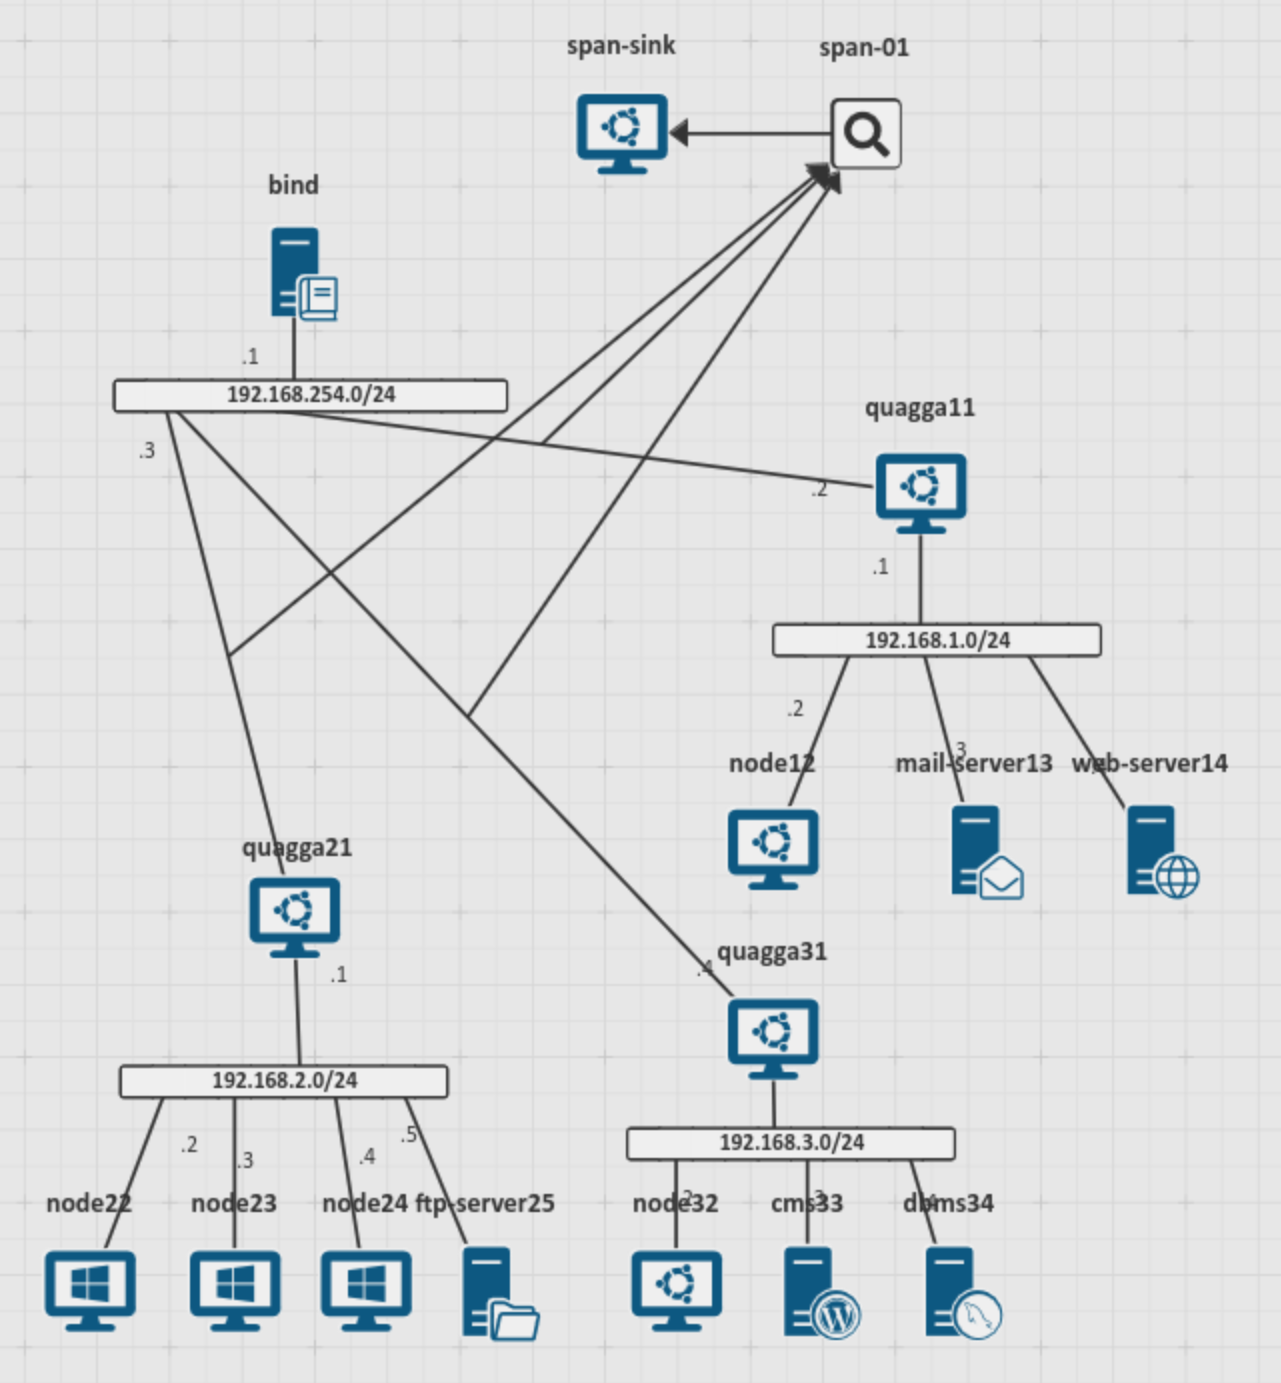
\includegraphics[width=\linewidth]{figures/topology.png}
    \caption{
      Example of a complete topology composed of 3 sub-topologies.
      Each sub-topology is connected to the rest of the network through a gateway.
      \label{fig:topologies.topology}
    }
  \end{subfigure}
  \caption{
    Topology generation with \thecontrib.
  }
\end{figure}


\subsubsection{Topology selection}

The topology selection is the most important part of the algorithm, as it requires finding all sets of sub-topologies that satisfy the user-defined constraints.
A sub-topology is composed of a subnet, a set of nodes (clients or servers), and a gateway that connects the subnet to the rest of the network.
\Cref{fig:topologies.example} shows an example of a sub-topology with 4 nodes.
Each sub-topology is formally defined as its \texttt{/24} subnet $s$, which also can serve as its identifier, and a set of clients $H_s$ and services $S_s$ that we generally refer to as nodes, \ie $N_s = H_s \cup S_s$.
The gateway $g_s$ is a particular node (not comprised in $N_s$) that connects the subnet to the rest of the network.
A sub-topology can therefore be represented as a tuple $t_s = \langle s, N_s, g_s \rangle$.
The topology selection is a \gls{csp} where the goal is to find all sets of sub-topologies that satisfy the user-defined constraints.
\Cref{def:csp} defines the concept of a \gls{csp}.

\begin{definitionbox}{\acrfull{csp}~\normalfont\cite{russell_Artificialintelligencemodern_2021}}{csp}
  A \acrfull{csp} is a tuple $P = \langle X, D, C \rangle$ where:
  \begin{itemize}
    \item $X = \langle X_1, X_2, \ldots, X_n \rangle$ is a set of variables.
    \item $D = \langle D_1, D_2, \ldots, D_n \rangle$ is a set of non-empty domains, one for each variable.
    \item $C = \langle C_1, C_2, \ldots, C_n \rangle$ is a set of constraints that specify allowable combinations of values in their domains.
  \end{itemize}

  Each constraint $C_j \in C$ is a new tuple $C_j = \langle \chi, R \rangle$ where $R$ is a relation between the variables in $\chi \subseteq X$.
  Thus, solving a \gls{csp} is finding an assignment of values for $X$ in $D$ that satisfies all constraints in $C$.
\end{definitionbox}

While dimensioning the output topologies can easily be translated using numerical boundaries, the constraints on the availability of services and attack scenarios in the sub-topologies are slightly more challenging.
We first define the service domain $D_\text{service}$ as the set of all services available in the library of sub-topologies, and tag each service node with its corresponding name, such as \texttt{ftp}, \texttt{postfix} (for email), or \texttt{ldap}.
An attack scenario is defined as another tuple $A_k = \langle \text{srcs} = \{N_1, N_2, \ldots\}, \text{targets} = \{N_{11}, N_{12}, \ldots\} \rangle $ where \texttt{srcs} and \texttt{targets} are sets of nodes available in the library that are compatible with the attack scenario.
For instance, a \gls{mitm} attack could be represented as $A_\text{MITM} = \langle \text{srcs} = \lbrace N_\text{attaker} \rbrace, \text{targets} = \lbrace N_1, N_2 \rbrace \rangle $.
Based on the aforementioned definitions, we can define our \gls{tsp} in \Cref{def:tsp}.

\begin{problembox}{\Acrfull{tsp}}{tsp}
  Given a set of sub-topologies $T = \{t_1, t_2, \ldots, t_n\}$, a set of services $D_\text{service}$, and a set of attack scenarios $A = \{A_1, A_2, \ldots, A_m\}$, find all sets of sub-topologies $T' \subseteq T$ that satisfy the following:
  \begin{enumerate}
    \item The number of sub-topologies in $T'$ is between $n_\text{min}$ and $n_\text{max}$.
    \item The total number of nodes in $T'$ is between $h_\text{min}$ and $h_\text{max}$. 
    \item Each service in $D_\text{service}$ is available in at least one sub-topology in $T'$.
    \item Each attack scenario in $A$ is compatible with at least one sub-topology in $T'$.
  \end{enumerate}
\end{problembox}

\subsubsection{Topology composition}

Once the sub-topologies are selected, the next step is to connect them to form a complete IT network.
The composition of the topologies is done in a tree-like structure, starting from the \emph{Master} sub-topology.
The \emph{Master} sub-topology is a special sub-topology that acts as the root of the tree and contains the necessary services to route traffic between the sub-topologies.
\Cref{fig:topologies.topology} shows an example of a complete topology composed of 3 sub-topologies.
At this point of the algorithm, the sub-topologies are already selected, and the composition is a simple matter of connecting the gateways while respecting the last constraint of tree-depth.
Yet, many variations of the same tree can be created, as illustrated in \Cref{fig:topologies.trees}.

\begin{figure}
  \centering
  \begin{subfigure}[b]{0.45\linewidth}
    \centering
    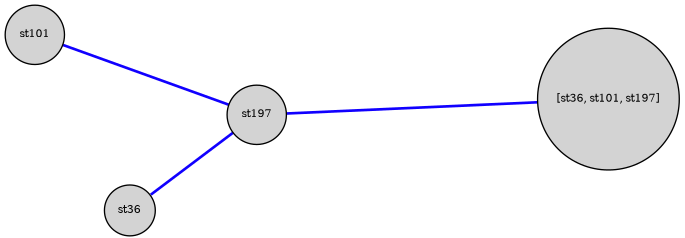
\includegraphics[width=\linewidth]{figures/graph3447.png}
  \end{subfigure}
  \hfill
  \begin{subfigure}[b]{0.45\linewidth}
    \centering
    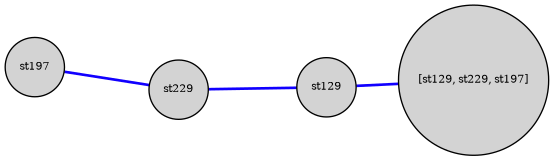
\includegraphics[width=\linewidth]{figures/graph3452.png}
  \end{subfigure}
  \hfill
  \begin{subfigure}[b]{0.45\linewidth}
    \centering
    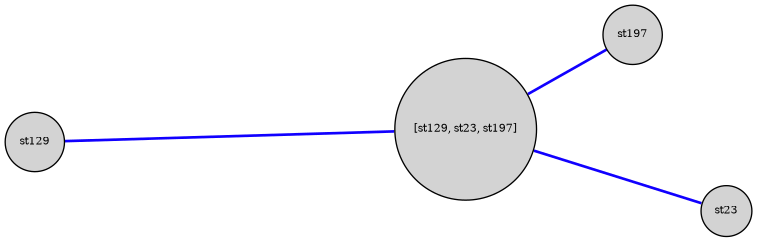
\includegraphics[width=\linewidth]{figures/graph3477.png}
  \end{subfigure}
  \caption{
    Examples of tree-like topologies composed of 3 sub-topologies.
    The \emph{Master} sub-topology is represented by the biggest node, and labeled with the IDs of the sub-topologies.
    \label{fig:topologies.trees}
  }
\end{figure}

\subsection{Implementation\label{sec:topologies.approach.implementation}}

In this section, we present parts of the implementation of \thecontrib using Airbus' CyberRange platform.
A CyberRange is a virtual environment that simulates a real-world network, allowing users to train and test their cybersecurity skills.
Most importantly, such platforms come with a set of templates that can be used to create sub-topologies, and compatible attack scenarios and user traffic generation tools to generate realistic traffic.
We implement or topology generator as a Python script that interacts with the CyberRange platform through its API to query the available sub-topologies, services, and attack scenarios.
The topology-selection algorithm is implemented using Google's \texttt{CP-SAT} solver\footnote{\url{https://developers.google.com/optimization/cp/cp_solver}}, and we develop a naive recursive algorithm to compose the topologies.
The constraints on the availability of services and attack scenarios are implemented as a simple filtering algorithm that removes sub-topologies that do not contain the required services or are not compatible with the attack scenarios.
We seed all random operation to ensure deterministic results.


\paragraph{The \emph{Master} sub-topology.}

The \emph{Master} topology serves as the basis for the composition.
It consists of a gateway connecting it to the Internet, a collection point for network logs, a DHCP server for distributing IP addresses, and a DNS server for resolving domain names across all topologies.
This is the only topology that will be configured, in particular to allocate the correct domain names to the IPs of the machines hosting the services that need to be accessible.
For example: web server (\texttt{webserver.local}), mail server (\texttt{mailserver.local}), file sharing (\texttt{fileserver.local}), etc.
This approach makes it possible to define unique domain names for each service, and make them accessible from any topology.


\paragraph{Handling connectivity.}

Now that all services are available via their domain names, the next step is to ensure that the services are reachable from any sub-topology.
To do so, each gateway $g_s$ hosts a DHCP server with a dedicated range to allocate IP addresses child sub-topologies.
The DNS configuration of the \emph{Master} topology is propagated to the DHCP server of each gateway, so that the domain names are resolved correctly.
To route traffic between the sub-topologies, the gateways also run an OSPF daemon to exchange routing information, announcing their own subnet to the rest of the network.
This setup allows to dynamically configure the routing tables of the sub-topologies upon deployment, and ensures that all machines are reachable.


\paragraph{Constraint satisfaction.}

As noted in \Cref{sec:topologies.approach.overview}, the topology selection is a \gls{csp} that can be solved using a constraint solver.
In particular, we implement our cardinality-related constrains (\ie, the number of sub-topologies and nodes) using the \texttt{CP-SAT} solver.
This generates all possible combinations of sub-topologies that satisfy the constraints, and we then filter out the ones that do not contain the required services or are not compatible with the attack scenarios.
The remaining sets of sub-topologies are then composed into complete topologies using a naive recursive algorithm that walks a tree, starting from the \emph{Master} sub-topology, and randomly assigns children sub-topologies to the gateways.
We implement a simple backtracking algorithm to roll back the composition when the tree-depth constraint is not satisfied, and try again from another branch.